\documentclass{article}
\usepackage{graphicx}
\usepackage{url}
\usepackage{array}
\usepackage[parfill]{parskip}
\usepackage[backend=biber, style=bath,]{biblatex}
\usepackage{hyperref}
\graphicspath{{./}}
\title{Flower Species Recognition on a Smartphone}
\addbibresource{refs.bib}
\author{Saahil Shihaz\\\\BSc Computer Science\\The University of Bath}
\date{May 2022}
\begin{document}
\pagenumbering{roman}
\maketitle
\clearpage
\begin{abstract}

Abstract goes here.

\end{abstract}
\clearpage
\tableofcontents
\clearpage
\listoffigures
\clearpage
\section*{Acknowledgements}
\thispagestyle{empty}

I'd like to acknowledge ...

\clearpage
\pagenumbering{arabic}
\section{Introduction}

This section will outline the overall plan for this dissertation, starting with an in-depth look at the problem and a 
brief look at the domain.

\subsection{Problem Description}

The technological era that we live in has introduced many ground breaking achievements that constantly push the barrier 
of what is possible as well as introduce many new challenges that require complex solutions. One such challenge is big 
data processing, specifically, recognising patterns in data and drawing conclusions. Unfortunately machines don't have 
the ability to understand data the way that humans do and humans don't have the processing capability of modern 
machines. Due to obvious ethical and biological barriers, we cannot make humans fill the role of computers that compute 
data on a large scale, therefore, we must explore the alternative, making computers as smart as humans. This is where 
machine learning steps in, with which we have made great advancements in. What this project will focus on in particular,
is granting the advanced capabilities of machine learning to lower end hardware.

\par

This project aims to investigate the application of machine learning techniques to recognize images of flowers species 
on mobile devices. I will look at implementing standard machine learning algorithms that are effective in image 
classification as well as alternative deep learning techniques which are more effective in carrying out the same task. 
It will be interesting to compare both types of implementations in terms of accuracy, speed and performance and then 
transferring them to a mobile hardware environment which is traditionally weaker than standard machines such as desktops
and laptops. Ultimately, we want to understand the best way in making a mobile software solution that can make use of 
machine learning methods and still maintain a seamless user experience.

\par

Mobile devices have the advantage of portability and flexibility compared to PCs at the expense of pure processing 
power, storage and battery life. Advancements in machine learning can boost the abilities of mobile devices by allowing 
them to make informed decisions to aid the user. Traditional algorithms can't make decisions like “What is this flower?”
without being cumbersome and inaccurate, we need something that can make good decisions and evolve, similar to human 
thinking. Smart phones and tablets are packed with more advanced technology than they've ever had like high resolution 
camera, sensors, displays and mobile processors, each of these are resources that a well written machine learning 
algorithm can take advantage of, for example, in our case, a mobile phone that can provide high resolution photos of 
flowers. The more detailed data we can use to aid our machine learning process, the better. 

\par

Traditionally, mobile devices as well as similar devices with sensors do some light pre-processing of data, then they 
send it to the cloud which can handle actions that require intensive processing, this introduces some level of latency 
because of the communication between device and the cloud (\cite{olascoaga2021hardware}, p. 3). 
Latency, being a key issue, is important in some use cases such as autonomous vehicles, mobile gaming, activity tracking
for vulnerable populations, etc (\cite{olascoaga2021hardware}, pp. 3-4).


\par

With some raw information, a (classical) machine learning process can identify features, these could be used by a 
classifier that can make predictions given a set of data it hasn't seen before (\cite{lecun2015deep}). Features are 
sourced from the representation of an object, in turn the representation is defined by the 
data input. An example of a feature would be the presence or absence of thorns on the stem of a flower 
(\cite{goodfellow2016deep}, p. 22). Traditional machine learning practices incorporated 
feature engineering that required designing custom algorithms for particular task which can be time consuming 
(\cite{liu2020representation}). There is also difficulty in understanding what features should be extracted, 
for example, it may be hard to represent flower petal shapes properly from raw pixel values if there are shadows being 
cast on it (\cite{goodfellow2016deep}, p. 23). Representation learning is a method that 
can fix such issues by providing mappings not from just the representation of data to the output, but from 
representation to representation (\cite{goodfellow2016deep}, p. 24). There are however, 
still hurdles to overcome, these are described as “factors of variation” where external factors might affect the source 
data, such as, the age of a flower, which could affect the petal shape and the season which may affect a flower's 
appearance. Factors like this make it difficult to get representations in the first place 
(\cite{goodfellow2016deep}, p. 24).

\par

Deep learning is a part of machine learning that aims to overcome limitations of classical machine learning techniques 
by expanding upon representation learning. Deep learning can be split into two unique parts:

\begin{itemize}
    \item \textbf{Distributed Representation:} These are used to represent objects within a more compact and dense manner, 
instead of having representations for each type of object, for example a collection of words in a sentence, we could 
store the frequency of each word like the bag-of-words problem (\cite{liu2020representation}). This is a sparse
representation and introduces problems with space and time complexity. Therefore distributed representations aim to 
tackle the sparsity problem as they are harder to model (\cite{Brownlee2017}).
    \item \textbf{Deep Architecture:} The idea of layering to represent neurons in a human brain. You can imagine it as a map of 
nodes that takes an input, processes it through the different layers where at each step, a set of units calculate a 
weighted sum of their inputs from the previous layer and pass the result to the next layer until it gets to output units
that generate a result. This is an example of a feedforward neural network (\cite{lecun2015deep}).
\end{itemize}

\par

Input into a deep learning algorithm starts at the visible layer, which contains our set of input pixels that we can 
directly observe. This data is passed into a network of hidden layers, each of these layers represent an abstract 
feature that we can't normally observe by looking at the input data such as locations of edges and contours 
(\cite{goodfellow2016deep}, p. 26).

\par

By making use of TensorFlow (Lite) we can produce classification models using languages like Python, C++ or Java, then 
convert said models into small packages that an Android/IOS application can use to generate predictions based on an 
input. TensorFlow is developed by Google and provides an machine learning based suite of tools to design, test and 
deploy ML solutions. The Lite version that we will be using is designed specifically for mobile devices and IoT devices 
that may not have the support of powerful hardware. Using TensorFlow we can write models that use classical ML 
techniques as well as deep learning techniques like Convolutional Neural Networks (CNN) (\cite{googleTF2}). 
There are examples that can be built specifically for flower classification within the API documentation which can serve
as a starting point for the project.

\subsection{Main Objectives}
\begin{itemize}
    \item Analyse existing mobile based image recognition software.
    \item Investigate the advantages and disadvantages of both classical ML and DL implementations and compare the two 
using analysis tools, this will be done on PC hardware.
    \item Design and implement an Android application that can recognize images using DL.
    \item Discuss the feasibility of DL on smartphones.
    \item Explore future improvements for the Android app.
\end{itemize}

\clearpage
\section{Literature and Technology Review}

Ground-breaking achievements in technology and specifically machine learning have given us the tools and capabilities to
tackle the key problem of image recognition. What this project aims to demonstrate is the application of deep learning 
within a mobile application to recognise flowers. It will be interesting to see how deep learning performs on mobile 
hardware which is generally less powerful than desktop PCs and laptops. Additionally, we will get to explore what sort 
of optimisations need to take place in order to get a feasible mobile based solution.  The limited computing resources 
that we have to work with when creating our solutions is what makes this project challenging. Mobile devices typically 
contain smaller mobile processors, limited storage and batteries. These restrictions are in place to 
make mobile phones more efficient and to ensure that they last longer when not connected to a power source. In addition
to this, the subject of machine and deep learning is complex and many find the concepts challenging to understand. 
What this literature review aims to do is identify key sources of information to help breaking down the underlying 
subject and discuss the quality of the research available.

\subsection{Mobile Machine Learning}

The potential of smartphones has still not been fully realised. With advancements in machine learning we can take the 
capabilities of smartphones to the next level by leveraging the advanced hardware within them to carry out complex 
tasks. This section will identify the key milestones within smartphone technology and how it leads us to integrating 
machine learning to make full use of the hardware.

\begin{figure}[h]\
    \centering
    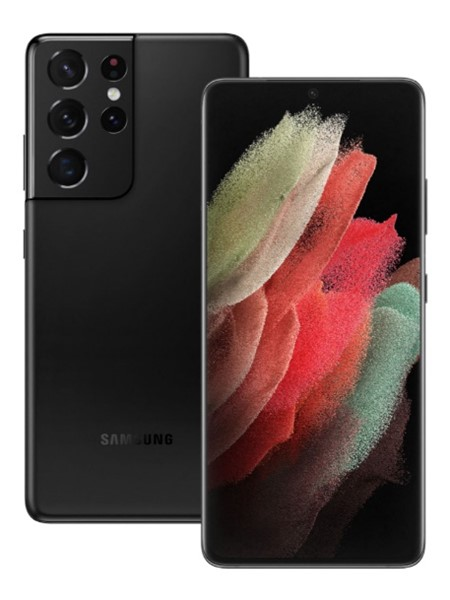
\includegraphics[width=0.3\textwidth]{s21ultra.jpg}
    \caption{Samsung Galaxy S21 Ultra 5G: Boasting an impressive array of camera sensors on the back (\cite{three2021}).}
\end{figure}

\subsubsection{Evolution}

Firstly, we want to look at the last 10 years of technological advancements within the smartphone space. 
With this information, we can hopefully gain some insight into the how much their capabilities have evolved. To do this, 
we will collect key aspects of specification data from the Samsung Galaxy flagship line of smartphones. Samsung 
currently hold the top spot in global market share at 20.8\% as of Q3' 2021, this position is typically held by Apple or
Samsung and can vary from a quarter to quarter basis (\cite{odea2021}).

\begin{table}[h!]
    \centering
    \begin{tabular}{ |m{2.5cm}|m{2.7cm}|m{1cm}|m{1.2cm}|m{2.5cm}| }
        \hline
        Phone (Year) & Processor & Storage (GB) & Memory (GB) & Cameras (MP) \\
        \hline
        \hline
        S2 (2011) & Dual-core 1.2 GHz & 32 & 1 & 8 \\
        \hline
        S3 (2012) & Quad-core 1.4 GHz & 64 & 1 & 8 \\
        \hline
        S4 (2013) & Octa-Core (4x1.6 GHz, 4x1.2 GHz) & 64 & 2 & 13 \\
        \hline
        S5 (2014) & Quad-Core 2.5 GHz & 32 & 2 & 16 \\
        \hline
        S6 edge+ (2015) & Octa-Core (4x2.1 GHz, 4x 1.5 GHz) & 64 & 4 & 16 \\
        \hline
        S7 edge (2016) & Octa-Core (4x 2.3 GHz, 4x 1.6 GHz) & 128 &	4 &	12 \\
        \hline
        S8+ (2017) & Octa-Core (4x 2.35 GHz, 4x 1.9 GHz) & 128 & 6 & 12 \\
        \hline
        S9+ (2018) & Octa-Core (4x 2.8 GHz, 4x 1.7 GHz) & 256 &	6 &	12/12 \\
        \hline
        S10+ (2019) & Octa-Core (4x 2.84 GHz, 4x 1.78 GHz) & 1024 &	12 & 12/12/16 \\
        \hline
        S20 Ultra 5G (2020) & Octa-Core (1x 2.84 GHz, 3x 2.42 GHz, 4x 1.8 GHz) & 512 & 16 & 0.3/12/48/108 \\
        \hline
        S21 Ultra 5G (2021) & Octa-Core (1x 2.84 GHz, 3x 2.42 GHz, 4x 1.8 GHz) & 512 & 16 &	10/10/12/108 \\
        \hline
    \end{tabular}
    \caption{All data is sourced from \cite{gsm}}
    \label{table:1}
\end{table}
\break
\clearpage

\par

We can see a clear increase in smartphone capability in multiple categories like the processor speed, core count, 
storage, memory and camera capabilities. There are of course may more different areas that are not listed like sensors, 
screen size and battery life which have also seen massive improvements over the last 10 years. We have only been seeing 
improvements in this space, therefore we can assume that we will continue to see improvements in the near future. 
What we must also consider is price and accessibility, flagship smartphones represent the top of the line offerings from
each smartphone manufacturer and are of course priced as such. Low-end to mid-end smartphones are still more capable 
than their predecessors albeit their spec sheet may not be as impressive as high-end versions in the same generation. 
Therefore, we must ensure some level of scalability within our machine and deep learning processes. How can we make 
sure our processes can run efficiently on lower end hardware as well as high end hardware?

\par

\citeauthor{kulendran2014} (2014), highlights how improvements in smartphones have created a boom in the number of 
smartphone based application designed to aid surgeons and patients in multiple facets of the medical industry like 
plastic, orthopaedic and general surgery. They conduct an expansive review of different solutions and analyse how the 
evolution of smartphones got them to the point that make them extremely useful as a tool to aid us. Ultimately, what 
this project aims to do is provide a robust software solution to recognise flower species on a smartphone, but we 
cannot ignore the fact that smartphones have come a long way in the hardware and operating system space to allow us to 
even conceive of a system.

\subsubsection{Where does this lead us to, today?}

ML and AI has become such an important part of smartphones that manufacturers now have dedicated processors for ML and 
AI tasks. Google includes a Tenor Processing Unit (TPU) in their Pixel line of phones (\cite{triggs2021}). Samsung, 
Qualcomm and Apple use their own solutions for machine learning processing by having their own bespoke processors. These 
processors are used to compute specific actions that require the decision making and accuracy capabilities of machine 
learning. Google Tensor in particular aids tasks such as speech recognition that is accurate but not taxing, therefore 
saving battery life. Tensor also applies to processing photographs and provides additional features to videos 
(\cite{gupta2021}). With such a focus on smartphones, to the point that they get dedicated hardware for ML, we should be 
seeing a huge increase in applications that integrate ML in some way, as well as the entire process of designing and 
implementing such solutions being carried out more rapidly, as developers learn to leverage the hardware.

\subsection{Computer Vision}

Since we are working with analysing images, the area of computer vision plays a big part in our research. In order to 
identify flower species we must first discuss techniques to analyse the incoming image data to make predictions using
ML and DL.

\subsubsection{History}

\citeauthor{SzeliskiRichard2011CV:A} (2011) outlines significant occurrences in each decade starting from the 70s, 
thought to be the beginning of computer vision, all the way through to the 2000s. In the early 70s, researchers sought 
to emulate human intelligence in a machine by first solving the visual problem. It was hypothesised that if a computer 
could first recognize objects in the real world that it could then move onto the next step of using reasoning and 
problem solving at a high level. The first processes conducted to understand the 3D world were to extract edges to 
recognize 3D objects from 2D lines in an image.

\par

The 80s were described to have a lot more focus on mathematical techniques for analysing scenes. Various algorithms 
and models were conceived as well as improvements in the contour and edge detection space. Researchers found that a 
lot of these algorithms could be thought of as “optimization problems” when they were described using the same 
mathematical framework.

\par

We see more improvements in the field during the 90s including the production of 3D surfaces, tracking and image 
segmentation. However, what is probably more relevant to this project is statistical learning techniques that also 
started to appear during this decade. In 1991, we see a paper by \citeauthor{turk1991face} (1991) that described
the concept of “eigenfaces”. These are the product of converting images of faces into feature images. These feature 
images are essentially the training set. Recognition occurs “by projecting a new image into the sub-space spanned by 
the eigenfaces”. The new face is then classified by comparing it's position relative to the known set of faces. 
Emphasis was placed on the limiting the scope of the allowed images, as such the system was trained and ready to 
accept profile straight-on images of the subject. In addition to that, they aimed to have the system compute a result
in a reasonable time, which of course, is one of the goals of this project. The research hoped to improve on it's 
predecessors that used, at the time, traditional methods of recognising features such as eyes', noses and mouths and 
their relative position to each other. The work done with eigenfaces shows great similarities with the machine 
learning techniques we see today, by essentially creating feature vectors and comparing the distance of known 
vectors in the same space.

\par

\citeauthor{SzeliskiRichard2011CV:A} (2011) continues with their insight into the 2000s where see the various 
improvements like more efficient algorithms and what finally dominates the latter half of the 2000s; applying machine 
learning techniques to computer vision to aid visual recognition research.

\subsection{Machine Learning}

This project will be using ML techniques to compare efficiency and accuracy to the more evolved deep learning. 
What we must first consider is how machine learning works in the context of computer vision. 
\citeauthor{CamastraFrancescoMLfA} (2015) summarise this and broke down ML development around three primary research 
points:

\begin{itemize}
    \item Task-Oriented Studies, improving performance of learning systems in a predetermined set of tasks.
    \item Cognitive Simulation, emulating the human brain and designing processes around the human thought process.
    \item Theoretical Analysis, “the theoretical investigation of possible learning methods and algorithms 
    independently of application domain”.
\end{itemize}

They also produce a taxonomy to represent the balance of two entities they describe: the “teacher” and the “learner”. 
The teacher, being the programmer, the one that designs the learning process and the learner being the computer system. 
The idea of inference is also introduced where a system can derive knowledge from previous observations. The taxonomy 
breaks down the amount of work that both the “learner” and the “teacher” need to do into four categories: Rote Learning,
Learning from instruction, Learning by analogy and Learning from examples.

\par

What we are more interested in is learning from examples where the “learner” infers the most out of the other 
categories in the taxonomy. The idea of the “learning problem” is introduced where the system needs to find a “general 
rule that explains the data given only a sample of limited size”. Learning techniques are broken down into four more 
categories: Supervised learning, Reinforcement learning, Unsupervised learning, Semi-supervised learning.

\par

\citeauthor{zhu2005semi} (2005) highlights semi-supervised learning in their survey as the combination of supervised and
unsupervised 
learning where we use both labelled and unlabelled data for training of the classifier. They point to the survey done by
\citeauthor{seeger2000learning} (2000) in particular that provides more insight into the concept of semi-supervised 
learning. Their rationale for the concept in general was applying the ability for a system to make predictions based on 
knowledge it doesn't have. A supervised system has all labelled data to aid it's training therefore it's basis on making
predictions is described as a “security belt” by Seeger. The model will basically make predictions within its limited 
scope, what we would call “overfitting” (\cite{tom1995}). Unsupervised learning heavily relies on prior assumptions for 
their final result this is because it doesn't have a knowledge base to rely on. By using a balanced combination of both 
implementations we can “balance the impact of prior assumptions”. Seeger also highlights the fact that labelling the 
data is a taxing process, fortunately for us, existing data sets already exist with labelled and unlabelled images for 
flower species which will be useful for training. Therefore, a semi-supervised approach is feasible for the ML approach
of this project.

\subsubsection{Feature Extraction}

\citeauthor{dishaa2021} (2021) provides an introductory guide to feature extraction. They describe feature extraction 
as one of the two ways to reduce dimensionality with the other being feature selection. Extraction produces new 
features which are described as “linear combination of the existing features”. The process aims to use less features to 
encapsulate the same image information.

\par

\citeauthor{tian2013} (2013) conducts a review of image feature extraction techniques that are worth considering. They 
start with discussing extracting colour features such as histograms and colour “moments” from specific colour spaces 
such as RGB and HSV. The paper also compares different types of colour features, for example, histograms are simple to 
compute but are sensitive to noise.  This feature will be important as flowers come in many different colours, but it 
cannot solely be relied on as different species can share similar colours. We can also extract information about 
the texture of an image, this is where we start thinking about analysing groups of pixels together. Texture in the 
context of images is a way to describe the perceived smoothness, roughness or bumpiness of an image though spatial 
variations in pixel intensity levels (\cite{mathworks}). Lastly, the paper goes into depth about shape features and 
points to different sources that go into the subject with more depth, but to summarise, shape features are 
split into two broad categories of contour and region based. This is where the features are calculated from shape 
boundaries and image regions respectively. A simple example of shape feature is the circularity ratio where you measure 
how close a shape is to a circle by calculating the ratio of the area of a shape to the area of a circle with the same 
perimeter (\cite{mingqiang2008survey}). Shape analysing will be very important in this project because flower shapes can
differ greatly and can therefore serve as a way to easily differentiate between species.

\subsubsection{Classification}

\citeauthor{brownlee2020} (2020) provides an easy-to-understand breakdown of classification within ML. They describe it 
as the process of assigning “a class label to example from the problem domain”. In our case, that means classifying a 
flower as species A as opposed to B, C or D. They also go into detail about the different classification methods such 
as:
\begin{itemize}
    \item Binary classification e.g. it's flower A or it's flower B.
    \item Multi-class classification, where we have more than two classes.
    \item Multi-label classification, this is where we have multiple predictions for classes based on a probability. 
    This can be a path we could take if we wanted to produce multiple predictions for a flower species and then provide 
    the likelihoods of each prediction to the user.
\end{itemize}
Next, we will look at classifiers, which help us carry out the classification stage. Fortunately, there is no shortage 
of types of classifiers in the ML space. \citeauthor{MohammedMohssen2017Ml:a} (2017) covers the most popular ones in 
good detail such as Naïve Bayes, k-Nearest Neighbour and Support Vector Machines (SVM). Starting with Naïve Bayes, this 
is a supervised classifier based on probability that assumes all attributes are independent:
\begin{equation}
P(c|E) = \frac{P(E|c)P(C)}{P(E)}
\end{equation}

Where \(E\) is classified as the class \(C = +\) if and only if
\[BC(E) = \frac{P(C = +|E)}{P(C = -|E)} \geq 1\]
\(BC\) is our Bayesian classifier, + and – are two separate classes (\cite{zhang2004optimality}).

\par

\citeauthor{zhang2004optimality} (2004) states that Naïve Bayes is superb in classification and demonstrates the
classifier based version of it in Equation 1. They explore the optimal conditions of Naïve Bayes and propose
that it is most optimal when the dependencies among attributes cancel out since Naïve Bayes works best when each 
attribute is independent, this is relevant as we want to explore optimisation in the project to ensure the highest 
level of efficiency when making the flower predictions.

\par

\citeauthor{MohammedMohssen2017Ml:a} (2017) states that K-Nearest Neighbours (KNN) is one of the “simplest” of  all the 
ML algorithms. \citeauthor{rosebook2016} (2016) discusses how to implement an image classifier using KNN where we can 
convert an image into a set of feature vectors on a graph, any new points get classified based on the k number of 
nearest neighbouring points, there's no real learning in this process, just the calculation of where the nearest points 
are, based on (usually Euclidean) distance.

\par

\citeauthor{NobleWilliamS2006Wias} (2006) describes SVM as a way to tackle binary classifications, which means in the 
context of flower classification it only really answers questions like “is it Flower A?”. They state that you would need
to train multiple “one-versus-all” classifiers. For this project, that may not be appropriate if we want to support a 
large number of flower species.

\par

ML techniques are certainly not useless and can still provide results, however, the research in the space has evolved 
to a new level, aiming to improve upon these traditional ML techniques in all evaluation categories. This is where Deep
Learning (DL) comes in.

\subsection{Deep Learning}

DL will of course be our alternative approach to recognizing flower species. Where ML is basically our baseline, our DL 
implementation should hopefully highlight how much better it is compared to the ML approach.

\subsubsection{Neurons and Perceptrons}

\citeauthor{ScarpinoMatthew2018Tfd} (2018) introduces the concept of Perceptrons in their book about using TensorFlow 
to implement DL. First, we must discuss neurons and how they relate to understanding the foundation of DL.

\begin{figure}[h]\
    \centering
    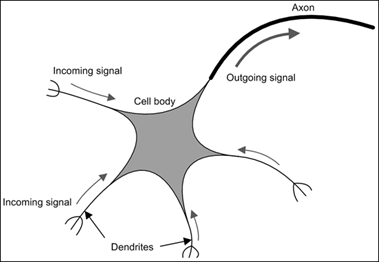
\includegraphics[width=0.6\textwidth]{neuron.png}
    \caption{Simple diagram of a neuron (\cite{ScarpinoMatthew2018Tfd}).}
\end{figure}

What they choose to highlight in particular are three points that describe a neurons functionality (and ultimately how 
it relates to perceptrons):

\begin{itemize}
    \item A neuron receives one or more incoming signals and produces one outgoing signal.
    \item A neuron's output can serve as the input of another neuron.
    \item Every neuron has a threshold, and the neuron won't produce output until its electricity exceeds the threshold.
\end{itemize}

This page by \citeauthor{anonpercep} (n.d.) highlights a brief history of perceptrons, though 
it serves a starting point to learn more about the concept. Perceptrons were coined by Frank Rosenblatt in 1962  
(\cite{rosenblatt1961principles}), though his research is a bit outdated for our analysis, therefore here is a 
more modern version:

\begin{figure}[h]\
    \centering
    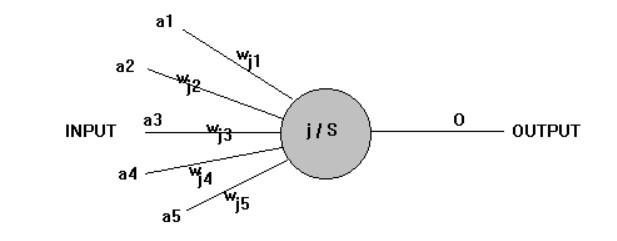
\includegraphics[width=0.7\textwidth]{perceptron.jpg}
    \caption{Diagram of a perceptron (\cite{anonpercep}).}
\end{figure}

Each input on the left is weighted and the summed within the circle node. If the summation meets a certain threshold, 
the output will be 1, if it doesn't meet the threshold then a 0 is outputted (\cite{ScarpinoMatthew2018Tfd}). 
Scarpino highlights some 
improvements to the model that was made including the weights that we discussed earlier as well as additional biases 
assigned with the incoming signals and an “activation function” that generates the output signal. Scarpino goes further 
by linking activation functions directly with in built TensorFlow functions that carry out the same task. Making it 
quite useful to understand the link between the TensorFlow API and the underlying DL context. Once we start linking 
perceptrons and arranging them into layers we get a neural network as shown here:

\begin{figure}[h]\
    \centering
    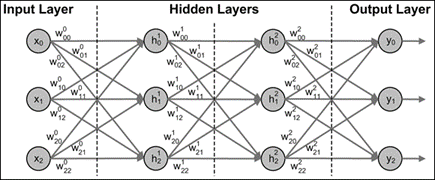
\includegraphics[width=0.7\textwidth]{network.png}
    \caption{Diagram of a layered network of perceptrons (\cite{ScarpinoMatthew2018Tfd}).}
\end{figure}

\subsection{Convolutional Neural Networks}
\label{subsec:cnn}

Bengio, Goodfellow and Courville (2015) and Scarpino (2018) go into detail about CNNs, Scarpino in particular is a
useful source on how it works with image classification in TensorFlow. However, it's useful to have 
some sort of starting point for the subject. \citeauthor{saha2018} (2018) highlights the key features of a CNN and their
purposes such as the individual layers: convolutional (kernel),  pooling and classification (see Figure 5).

\begin{figure}[h]\
    \centering
    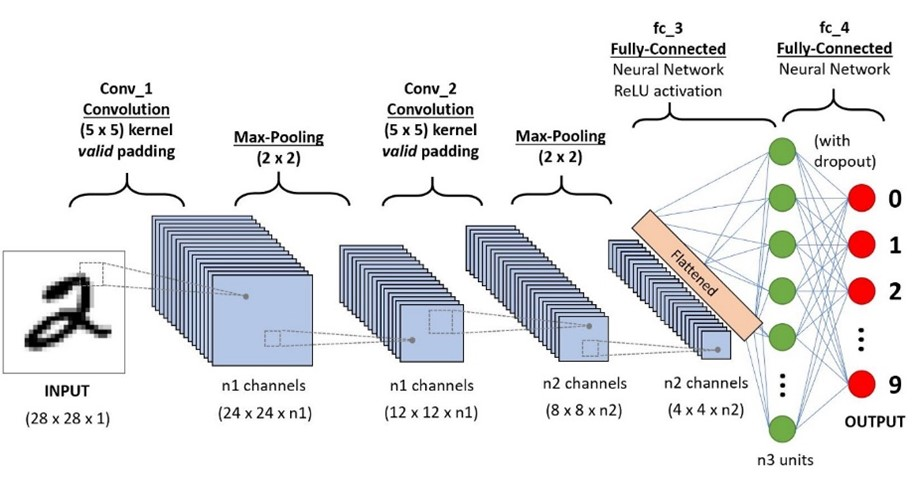
\includegraphics[width=0.7\textwidth]{saha.jpg}
    \caption{Example of a CNN process (\cite{saha2018}).}
    \label{fig:cnnSimple}
\end{figure}
\break

They also highlight a feature of CNNs that make images easier to process, where it reduces the size of images “into a 
form that is easier to process, without losing features which are critical for getting a good prediction”. This helps 
with our scalability approach when it comes to dataset sizes in particular. The ELI5 (Explain Like I'm 5) format is 
quite useful and allows us to highlight the key points of each layer (Saha, 2018):

\begin{itemize}
    \item Convolution: Applying the kernel to extract high and low level features.
    \item Pooling: Reduces the spatial size of the output from the convolution. Decreases the “computational power” 
    needed for data processing. Additionally, highlights features that are dominant.
    \item Classification: The pooling output is converted into column vectors and fed into a feed-forward neural 
    network where the model is able to distinguish between features and classify them.
\end{itemize}

Saha (2018) also highlights that there are actually different implementations of CCNs, therefore they may not function 
in exactly the same format. Dive into Deep Learning (\cite{diveintodeeplearning}) has a run down of multiple CNN types 
starting with LeNet-5 and more modern approaches like AlexNet, VGG, NiN, GoogLeNet, etc. We can also see how to 
implement them using TensorFlow which will prove useful when implementing our own solution for flowers.

\citeauthor{goodfellow2016deep} (2015) go into detail about Deep Learning from the concept of perceptrons to modern 
implementations. Something they talk about that is interesting is the increasing data set and model sizes over time, 
which is quite applicable to the project since we are working with modern mobile hardware. They discuss how the 
increasing capabilities of computer hardware have led to the development of larger models and that neural networks tend 
to double in size roughly every 2.4 years. They predict that the trend will continue further on in the future. What is 
also relevant is the dataset sizes. Storing datasets take up storage space, they state that a deep learning algorithm 
(as of 2015) is stated to perform at acceptable levels with “around 5,000 labelled examples per category, and will match
or exceed human performance when trained with a dataset containing at least 10,000,000 labelled examples. That is of 
course, extremely large and is most definitely going to take up a lot of storage. Therefore, the book does re-iterate 
the earlier point of making use of unlabelled data like with semi-supervised learning. \citeauthor{goodfellow2016deep}
(2015) dig deep into the subject of DL and explain subjects from the applied maths to the modern practices of DL and 
the research in the field. This can prove useful in fully understanding the various processes in place including 
optimisations and ways to increase accuracy that we will need to consider when designing a DL model for the mobile 
application.

\subsubsection{ML vs DL}
\label{subsec:mlvsdl}

DL is an obvious evolution from ML, but it is worth highlighting the key differences for clarity because ultimately this 
project will compare how ML and DL compete with each other. \citeauthor{kav2020} (2020) breaks down how DL is different 
from ML. They highlight that DL takes the initiative by automating feature extraction to lessen human intervention and 
that ML is more reliant on humans, where humans normally define the characteristics to look out for, as well as their 
priorities. DL is stated to “require more data points to improve its accuracy” compared to the ML counterpart.

\par

\citeauthor{8359287} (2018) goes into depth about the key differences when discussing approaches to ML and DL in the 
context of cybersecurity. However, the same reasoning can be applied in our situation. The key points they highlight 
are:

\begin{itemize}
    \item Data dependencies: DL performs better with larger datasets like mentioned earlier as well as ML 
    outperforming DL with smaller data sets.
    \item Hardware dependencies: DL requires a lot of matrix calculations and therefore a Graphical Processing 
    Unit (GPU) can be used to optimise these processes. Note that mobile hardware do contain GPU hardware but they are
    not on the same scale as dedicated GPUs you find in PC hardware. Therefore, it will be interesting to see how DL 
    fares against ML when we keep this hardware dependency in mind.
    \item Feature processing: Once again iterating on the point mentioned before, DL can extract features directly 
    from the data and requires less human intervention.
    \item Execution time: DL algorithms take a lot longer to train compared to ML, this is dependant on the amount of 
    data.
    \item Interpretability: Because of the complexity of DL it is hard to determine how a DL algorithm generated a 
    result, whereas ML is more clearer.
\end{itemize}

I have summarised the key points, but they go into much more detail which could be helpful in the evaluation stage 
of comparing the two approaches of ML and DL.

\subsection{Flower Classification}

We will discuss further how flower classification is carried out including the use of ML and DL techniques, what 
features are extracted, the datasets that are used and the key challenges.

\subsubsection{Existing Methods}

Starting with what is known as the “Hello world” of ML, Iris flower classification serves as a simple and easy to 
understand project for developers to implement. The idea is to classify between three classes: Versicolor, Setosa and 
Virginica. There are many tutorials that can be followed online, this particular one by \citeauthor{DataFlairND} (n.d.) 
provides additional background information about ML as well as how it will apply to the Iris project which is useful for
our understanding. The tutorial uses the features of sepal length/width and petal length/width to determine the class of
a flower. By using those inputs, they use a SVM to predict the species of a flower with 96\% accuracy. I mentioned 
earlier that it may not work well for a large number of species, but it certainly works well for a small number of 
classes.

\par

\citeauthor{Nilsback2008} (2008) demonstrate the effectiveness of a multiple kernel SVM on the oxford flowers 17 dataset. 
They manipulate the flower data to get key features such as the colour HSV values, the flower texture, shape and 
histogram of gradients (HOG) which “captures the more global spatial distribution of the flower” like the where the 
petals are arranged. They achieved an accuracy of around 88.3\%. This is impressive considering the key challenges they 
highlight within flower classification. They state that flowers can share a lot of similarities between classes which 
can make it difficult to differentiate between species. Flowers are also “non-rigid objects” and therefore can appear in
many different variations. Overall, they do a good job of explaining their reasoning for their dataset, citing the 
large variation of representations for each flower, and how they extract features from it, as well as how to build the
classifier.

\par

For deep learning, there is an extensive study that looks at using transfer learning, which is a technique of retraining
TensorFlow models for different data sets. \citeauthor{Xia2017} (2017) use the Inception-v3 model to train a classifier for 
the Oxford-17 and Oxford-102 flower datasets. They go into detail about the steps that took place to carry out the 
transfer learning as well as how to reconfigure the last layer of the network to only have 17 and 102 outputs for each 
dataset as it defaults to 1000. They found that the model for the for Oxford-17 and Oxford-102 datasets 
produced 95\% and 94\% accuracy respectively. This is very impressive performance, and their breakdown will be helpful 
when it comes to my own implementation. The paper really outlines the simplicity and flexibility of the Google's 
TensorFlow, however, we will still need to investigate if these great results will translate to a mobile implementation 
as well.

\subsubsection{Existing Apps}

A large part of the project is to develop a fully functioning app that is developed to be more like a commercial product
in addition to using deep learning techniques for the flower classification. This means developing features that will 
aid the user with using the app outside of main use case of recognising flowers. We will look at existing solutions that
are already real products used by real people.

\par

Pl@ntNet is a popular tool that has more than 10 million downloads on the Google Play Store alone (\cite{googleplay}). 
It relies on volunteers to validate images and a search engine to identify them. \citeauthor{joly:hal-01182775} (2015) 
go into detail about the overall experience of the app as well as provide insight into how it works.

\begin{figure}[h]\
    \centering
    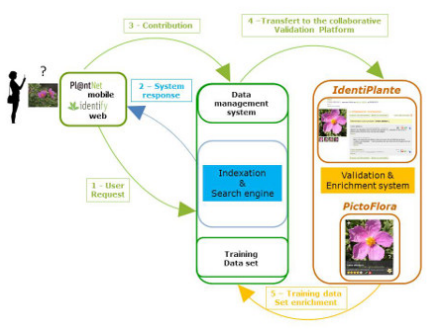
\includegraphics[width=0.7\textwidth]{plantnet.png}
    \caption{Diagram of Pl@ntnet user scenario (\cite{joly:hal-01182775}).}
\end{figure}

Figure 6 shows clearly the type of system in place for the application. The user uses their device to query the search
engine and get feedback, their image is also transferred to the collaboration platform if they chose to. It can then be 
independently verified and added back to the training set. The search engine is then retrained on a nightly basis. The 
paper doesn't go into much more detail about the search engine itself apart from mentioning that progress in machine 
learning and computer vision should improve the performance of identification. Unfortunately, there aren't any new 
papers that provide a better look at the app, so it is hard to understand what changes have been made over the last 
several years as well as how what methods they use to build the search engine. There is however, a dataset now 
available for use that covers over a thousand plant species with over 300 thousand images 
(\cite{camille_garcin_2021_5645731}). This is of course out of the scope of the project as it doesn't strictly contain 
flowers, but it does go into detail about how to use the dataset as well as how to load the data and build a model with 
it.

\begin{figure}[h]\
    \centering
    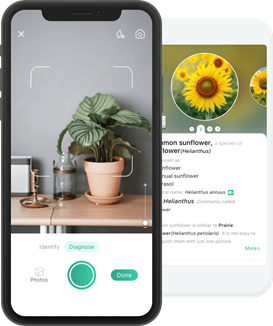
\includegraphics[width=0.5\textwidth]{picturethis.png}
    \caption{Screenshot of PictureThis app (\cite{picturethis}).}
\end{figure}

PictureThis is another plant identification app (shown above) that doesn't go into detail about how it works but does 
note that it requires an internet connection to function properly. This suggests that it must communicate with a server 
in order to generate a prediction for images. The app is very streamlined and has an easy-to-use UI that also contains 
useful features such as how to care for the plant and important information about it. My approach will be different in 
the sense that any identification process will be carried out on the device, however, it is still important to consider 
alternative methods and how they perform, so that we can compare approaches.

\subsection{Evaluation}
\label{subsec:evaluation}

One of the key points of the project is having to evaluate the ML and DL approach, what we haven't discussed 
yet however, is how do we go about doing this?

\par

\citeauthor{10.1145/1163593.1163596} (2006) identify a process named “k-fold cross validation” where the data set is 
“divided into k subsets”. One of the subsets is used to test the classifier and the rest (k-1) subsets is used as the 
training set. They use three performance metrics to test their ML systems: accuracy, precision and recall. Accuracy 
being the percentage of correct decisions over the total number of test instances. Confusion matrices can help us with 
representing accuracy by providing a “summary of prediction results” where we use the count of accurate and inaccurate 
predictions per class to show which particular classes the classifier may be struggling with (\cite{Brownlee2020b}). 
Precision and recall are a bit more complex. 
Fortunately, \citeauthor{shung2018} (2018) demonstrates how these two differ to accuracy. Precision is the number of 
instances that are correctly determined over the total number of instances that are guessed, this is made up of 
correctly guessed instances as well as instances that are incorrectly guessed. Recall is the number of correctly 
predicted instances over the true number of instances in the class. In addition to these evaluation methods, 
\citeauthor{10.1145/1163593.1163596} (2006) outline measuring CPU and memory usage. Fortunately, TensorFlow (lite) 
contains benchmarking tools for us to measure: Initialization time, inference time of warmup state/steady state, memory 
usage during initialization time and overall memory usage (\cite{googleTF}). I will also assess real world speed and 
accuracy by analysing the app's performance during development. The TensorFlow (lite) guide also contains tutorials on 
how to choose the best model for the task by comparing model size and accuracy of different models as well as the time 
it takes to make the prediction. The lite version is designed specifically for mobile and internet of things (IoT) 
hardware, so the additional tools will prove useful for the project later when we are at the evaluation stage.

\par

\citeauthor{Chockwanich} (2019) use the same evaluation methods outlined when comparing different DL models 
implemented in TensorFlow. They also look at CPU usage percentages and processing time. They were able to make a clear 
conclusion of which model is better by evaluating all factors. A term called f1-score was also mentioned in their 
analysis. Shung (2018) also explains the relevancy of f1 score, it is essentially a way to determine a “balance between
precision and recall”. \citeauthor{kors2021} (2021) discusses the F1 score and it's purpose in providing a better 
accuracy statistic that accounts for “imabalanced data”, this is when you don't have a good balance of data for each 
class and therefore the classifier makes inacurate predictions heavily skewed towards classes you have more data for. 
The F1 score is calculated by:
\[\frac{2*Precision*Recall}{Precision + Recall}\]

\subsection{Summary}

The review has highlighted the progression ML and DL from the early concepts and how everything eventually fit 
together to form what we know today. The area will keep getting more exciting as we learn to optimise our current 
algorithms, come up with new ones and make use of advancing hardware capabilities. ML and DL is getting more and more 
accessible as manufacturers allow the use of their specialised hardware to developers who can make use of APIs built 
specifically for these tasks. Overall, we have built on the solid foundations of previous research and it's interesting 
to see how the field develops in the future. The project hopes to aid the field by investigating the ML and DL 
approaches in the mobile format as well as explore why we see certain results from the evaluation.

\clearpage

\section{Investigation}

The main body of this dissertation will be split into two sections: the first being an analysis of TensorFlow's deep 
learning python API and how it compares to traditional machine learning python libraries like scikit. The second being 
the design and development of the flower classifier app. We will start with the investigation portion of the project,
walking through my initial predictions, methodology and findings. The idea is to approach this investigation from the 
perspective of a software developer that is analysing the best approach for method of flower classification to use in 
their product. This includes assessing the quality of the resources available and discussing the possible challenges.

\subsection{Predictions}

The main prediction is that implementing a convolutional neural network is more suitable than using classical machine 
learning methods for this task. Suitability will be judged based on the metrics described in section
\ref{subsec:evaluation} Evaluation. Furthermore, the process of implementing 
both approaches and the challenges that were faced will be described. Additional predictions mainly align with what was 
found in subsection \ref{subsec:mlvsdl} when discussing the key differences between ML and DL.

\subsection{Design of Experiments}

In this section, the implementation of the ML and DL classifiers will be individually described. The results from each
approach will then be compared to fully understand the advantages of DL over ML. Furthermore, the development process
including the various challenges faced will be discussed.

\subsubsection{Oxford Flowers 102 Dataset}

This dataset consists of 102 different flower species that occur within the UK. Each class contains between 40 and 258 
images each. The images are described to have large variations between scale, pose and lighting, even within the classes
itself. First the dataset will be downloaded and managed by the TensorFlow Datasets module (TFDS) which will download 
the dataset to a generic directory and can directly manage the image and dataset data including filenames, class names 
and data splits. The data splits defined by TFDS consists of 6,149 images for the test set and 1,020 images for the 
train and validation sets each. This split is atypical as you would ideally have a larger number of images in the train 
set rather than the test set. The current split is thought to be a mistake on Google's side (\cite{githubissue}). As a 
result, I will swap the train and test datasets and carry out the training process with the larger split which would be 
75\% of the dataset (\cite{TFOX102}).

\begin{figure}[h]\
    \centering
    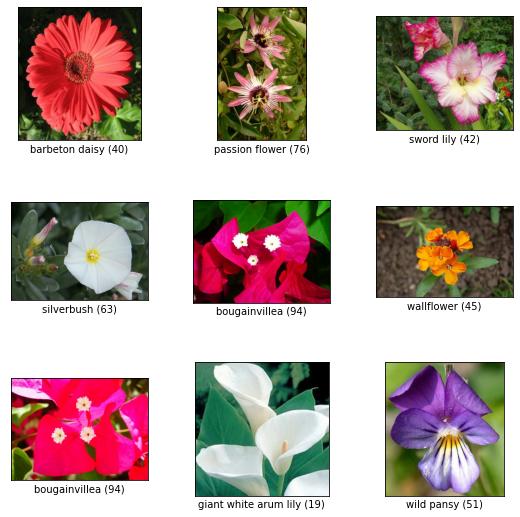
\includegraphics[width=0.7\textwidth]{ox102examples.png}
    \caption{Example images from the dataset.}
\end{figure}

\subsubsection{Classical Machine Learning}

For this approach I decided to go with a Support Vector Machine (SVM) classifier that takes in features generated using 
“bag-of-words”, HSV (Hue, Saturation, Value) colour values and histogram of gradient values. I went with SVM because 
good performance has already been achieved with this particular dataset before with \citeauthor{Nilsback2008} (2008) as 
stated in the 
literature review. A value of 98.5\% accuracy has also been achieved be using a CNN to extract the features 
(\cite{mete}). I will not use a CNN to extract the features as the purpose of this investigation is to evaluate both 
approaches separately instead of combining aspects from both. Bag of words will be used as it is simple to implement, 
but will also provide consistent information about key points found in the image, despite how the image is presented in 
terms of factors like rotation and scale (\cite{mohan}). By using an additional library named cv2, we can use a K-Means 
trainer to produce feature clusters. The “words” will be produced by extracting key points using Scale Invariant Feature
Transform (SIFT). HSV values are useful as they give us the relevant colour data as well as information about the 
luminance in the image (\cite{chapelle1999support}). Histogram of gradients values provide information about the general
shape of 
the object; this is useful in mapping the various shapes and sizes that flowers come in. The words will then be 
clustered by the trainer and make up the “vocabulary”. The dataset images will be resized to have a height and width of 
299 pixels to match the input image conditions of the deep learning approach. All SVM parameters will be set to the 
default that is defined by the documentation.

\subsubsection{Deep Learning}

The CNN used in this approach will be Inception V3, a pre-trained network, specifically trained on the iNaturalist 
dataset, which contains 675,170 training and validation images from 5,089 categories (\cite{paperswithcode}). 
This means that the model has been optimised for recognizing plants and animals which makes it the best candidate to be 
used for transfer learning to allow it to recognize flower species. It is also listed as the second-best model hosted on
TensorFlow. Inception V4 exists and has better performance to V3 but there are no fine-tuneable V4 models available that
will allow transfer learning to take place.   

\begin{figure}[h]\
    \centering
    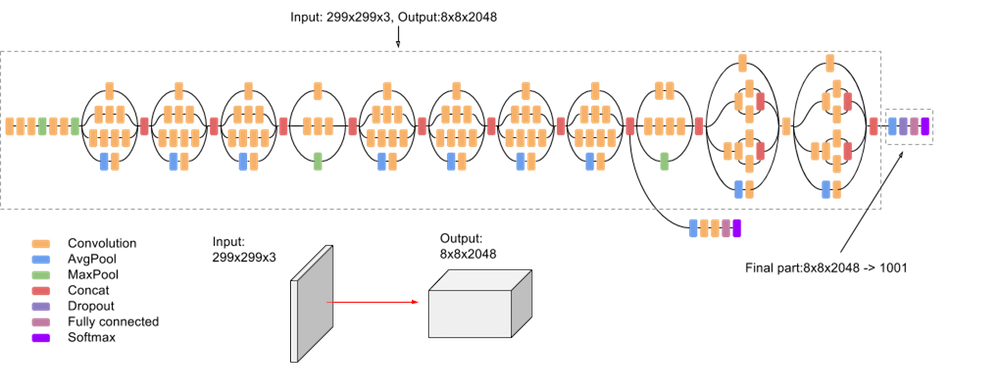
\includegraphics[width=\textwidth]{inceptionv3.png}
    \caption{The Inception V3 model diagram (\cite{GoogleCloud}).}
    \label{fig:inception}
\end{figure}

Compared to the initial research of deep learning models presented in figure \ref{fig:cnnSimple} within the literature 
review, figure \ref{fig:inception} demonstrates how complex deep learning models can truly be. 
We discussed the terms convolution and pooling within section \ref{subsec:cnn}, however there are additional layers here that were 
not discussed:

\begin{itemize}
    \item Concatenate (Concat) takes a list of tensors and outputs a single combined tensor (\cite{kerasconcat}).
    \item Fully connected layers map all inputs in the previous layer to every “activation unit” of the layer next to it
(\cite{singhsurya}).
    \item Softmax is where probabilities are assigned to each label based on the likelihood of the image belonging to 
that label. All probabilities add up to 1 (\cite{googledevcnn}). 
    \item Dropout mitigates overfitting of a dataset by randomly dropping out neurons on each pass of the network when 
    training (\cite{seb}). 
\end{itemize}

The images will go through some data pre-processing such as resizing to have a width and height of 299 as that is the 
requirement of the input tensor for Inception V3. They will also have to have their values rescaled from 0-255 to 
between 0-1. Random flips and crops will also be added as part of the pre-processing pipeline. Images will be batched 
into sets of 32 images, this means that 32 images will be trained per step per epoch. Hyper parameter tuning is also 
required to try and get the best performance possible. These are the hyper parameters will be adjusted and
their supposed effect:

\begin{itemize}
    \item \textbf{Optimiser} is used to improve the speed and performance the model by adjusting the parameters of the 
    model during training to minimise loss and maximise accuracy. (\cite{maithani}). The types of optimiser that will be
    tested are Adam, Stochastic Gradient Descent (SGD), AdaMax. There are a few more optimisers 
    available that are not listed, as they are unsuitable for this dataset.
    \item \textbf{Learning rate} is the rate at which a model learns, a larger value means that the model learns faster 
    at the expense of producing substandard weights for the model (\cite{andreaperlato}). Values from 0.01-0.0001 will
    be tested, moving down a magnititude at each step. 
    \item \textbf{Dropout} which was described earlier when discussing the Inception V3 model. Increasing this value 
    will mean a larger percentage of nodes will get removed. Values within the range 0.2-0.4, in increments of 0.1 
    will be tested.
\end{itemize}

Using a TensorFlow module called TensorBoard, we can test the hyper parameter combinations efficiently and produce the 
metrics for each combination. TensorBoard allows the developer to view how the hyper parameters affected the results. 
In an effort to decrease overall training time and save time, I will conduct some preliminary testing to see which 
optimiser is more suitable with just baseline parameters. Once that is selected, I only need to test the different 
learning and dropout rates using a grid search. This is when every possible combination is tested. When testing with a 
large number of hyper parameters, one can use other methods like random search to decrease overall tuning time by 
randomly sampling hyper parameters from a range based on a statistical distribution, this means that more effective 
hyper parameters are tested to avoid spending time on hyper parameters that will not affect the overall performance that
much (\cite{sayak}). 

\subsubsection{Environment}

\label{subsec:env}

Both approaches will be developed and ran on the same machine, a custom desktop PC that contains these main components: 

\begin{itemize}
    \item An AMD Ryzen 3600 4.2Ghz 6 Core/12 Thread CPU
    \item 16GB 3200Mhz DDR4 Memory
\end{itemize}

The PC ran on Ubuntu 20.04 LTS with the relevant python3 and TensorFlow libraries needed to run the Jupyter Notebooks 
locally. VS Code was used as the Integrated Development Environment (IDE) with the Python and Jupyter extensions.  It is
possible to run model training on the GPU instead of the CPU, however, only Nvidia GPUs are directly supported. As a 
result of not having access to one, we will be mainly using the power of the CPU to carry out training.

\subsubsection{Metrics}

The key metrics I will analyse along with accuracy, precision, recall and F1 are: 

\begin{itemize}
    \item Loss, a measure of how bad the model's predictions are (\cite{googletrainloss}). 
    This metric only applies to the deep learning model as it is calculated during the training process as the model 
    tries to minimise it.
    \item Area under the receiving operating characteristic curve (AOC). You get an ROC curve by plotting the true 
    positive rate against the false positive rate. The area under this curve indicates how well the model is selecting 
    the correct prediction against all other predictions (\cite{googleroc}).
\end{itemize}

\subsubsection{Results}

\subsubsection*{Preliminary DL Findings}

Another factor to consider when carrying out training is the number of epochs. An epoch is a full pass over the training
set. Multiple passes are needed to minimise loss and fully train the model. Through preliminary testing of the model, 
I found that 5 epochs are more than sufficient as we reach the maximum validation accuracy shown in figure 
\ref{fig:incep_acc}. If we 
increase the number of epochs, we risk overfitting (\cite{geeksforgeeks}). Optimisers were tested individually to 
determine how much they would affect the results under standard conditions. I found that SGD was unsuitable for this 
task, producing accuracy results at almost half of what Adam and AmaMax were producing. Overall, Adam produced the best 
results, albeit AdaMax was only a percentage point behind. Therefore, I decided to conduct any main hyper parameter 
tuning, purely using the Adam optimiser. All initial training is done to only the first epoch to reduce overall 
execution time. 

\begin{figure}[h]\
    \centering
    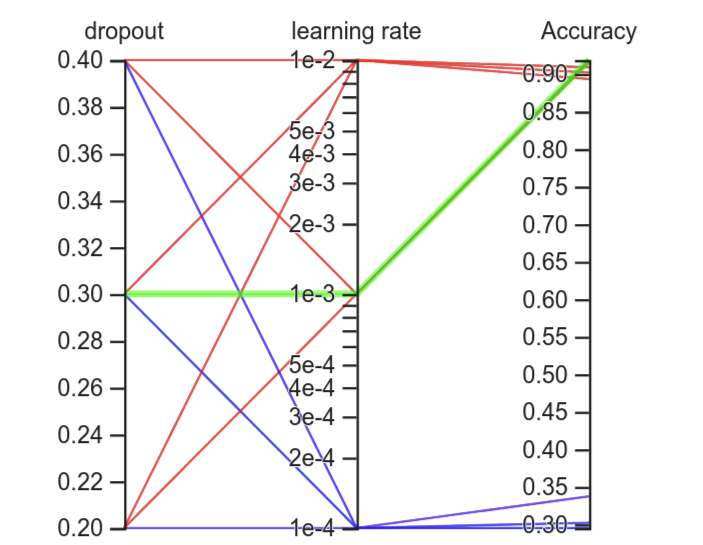
\includegraphics[width=0.6\textwidth]{cross_graph.png}
    \caption{Graph generated in TensorBoard from HP training results.}
    \label{fig:cross}
\end{figure}

\break

Figure \ref{fig:cross} above is a parallel co-ordinates view shown within TensorBoard that clearly show what accuracy 
results 
certain combinations of hyperparameters produce. Highlighted in green shows the joint first highest with a dropout of 
0.3 and a learning rate of 0.001. A dropout of 0.2 with the same learning rate produces the same result. A learning rate
of 1e-4 produces a significant reduction of first epoch performance, this is because we would need to increase the 
number of overall epochs to get optimal results. Ideally, we would test the number of epochs along with the other 
hyperparameters to produce fairer results, however, that would significantly increase training time with a grid search. 
If a developer has access to more specialised hardware, suited for machine learning tasks, this would not be too much of
an issue.

\par

Overall, the final model will use a learning rate of 0.001 and dropout of 0.3. This was decided after considering the 
results from the hyper parameter tuning (Appendix \ref{subsec:hp}) as well as the proposed learning rate being the 
default one provided by the TensorFlow API.

\subsubsection*{Performance}

\begin{table}[h!]
    \centering
    \begin{tabular}{ |m{3cm}|m{3cm}|m{3cm}| }
        \hline
        Metric & SVM (\%) & Inception V3 (\%) \\
        \hline
        Accuracy & 24.30 & 95.69 \\
        \hline
        Loss & - & 17.95 \\
        \hline
        Precision & 29.40 & 96.14 \\
        \hline
        Recall & 24.30 & 95.69 \\
        \hline
        F1 & 26.60 & 95.91 \\
        \hline
        ROC AUC & 89.60 & 99.97 \\
        \hline
    \end{tabular}
    \caption{Results output from the classifier after predicting against the testing dataset.}
    \label{table:2}
\end{table}

Precision, recall and ROC AUC values are weighted, meaning that they consider class balance as they calculate the metrics
for each class and find the average weighted by the number of correct instances for each class 
(\cite{scikitprec}). This was necessary to account for the slight imbalances we have with the number of images 
in each class. The deep learning approach clearly comes out on top with excellent results.

\par

The Inception V3 test contains additional information about accuracy (figure \ref{fig:incep_acc}) and loss 
(Appendix \ref{subsec:loss}) for the training and validation datasets 
while the model is being trained. It tells us how the model improves per epoch.

\begin{figure}[h]\
    \centering
    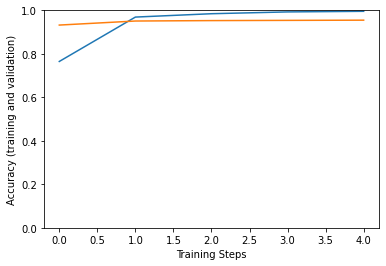
\includegraphics[width=0.6\textwidth]{inception_acc.png}
    \caption{Graph of accuracy against the number of training steps.}
    \label{fig:incep_acc}
\end{figure}

The model needs to be converted to a TensorFlow lite file in order for it to be allowed to be used in the Android 
application. Once we convert it, we can reload the model and run inference on it to check if it is still effective. The 
result after doing that produces an accuracy of 100\% if we just test it on the first batch of 32 images. Of course, 
his is not indicative of real-world performance, and we will need to do additional real-world performance profiling 
once the app is developed. 

\subsubsection{Analysis}

\subsubsection*{Outcome}

It is clear that the DL approach is vastly superior in classifying flowers than the SVM in all aspects. The Inception V3
approach has high accuracy meaning it can correctly identify the classes of most of the images in the test set. 
High precision indicates that a large portion of correct identification were genuinely correct. High recall demonstrates
how well the classifier identified correct instances. You might notice that accuracy and recall are the same value for 
both classifiers, this is because they represent the same thing in non-binary classification. Recall is shown to be:

\begin{equation}
    \frac{TP}{TP+FN}
\end{equation}

Where \(TP\) is number of true positives and \(FP\) is the number of false negatives (\cite{googledevrecall}).

\par

In this case, FN is every incorrect evaluation of a class. Therefore, if you calculate this recall value for each class,
you're essentially tallying up the number of times the class has been correctly identified over the total number of 
images in the class for every class, giving us the total accuracy. F1 gives us a better indication of the accuracy of 
the classifier, by taking into account the precision and recall, the high F1 score indicates that even with class 
imbalance, we get good classification results. An AUC of near 100\% means that the predictions are nearly always 
correct. The other predictions of an image are taken into account, so while the classifier might choose the incorrect 
overall label, if the true label has a high probability, this means that the classifier is still somewhat good at 
identifying the correct label.

\par

The SVM falls behind in every aspect, therefore, it is not worth pursuing as a method for flower classification in this 
dataset. It is still possible to adjust the parameters of the SVM to get better performance or get more feature data 
from the feature extraction methods. The current implementation, specifically the histogram calculations, use parameters
that decrease extraction and training time significantly, in exchange for outputting less information. 
\citeauthor{Nilsback2008} (2008) 
achieved an accuracy of 88.3\% with the oxford flowers 17 dataset, a smaller subset of the one being used here using 
very similar methods of combining SIFT, HOG and HSV and using an SVM. Their method is a lot more intuitive than my SVM 
implementation but still doesn't reach the performance of the Inception V3 model. This doesn't mean that SVM or any 
other classical machine learning method is obsolete, even in being used as a classifier on mobile phones. They can still
perform extremely well on smaller and less complex datasets. Therefore, if dataset complexity is not an issue, what 
else is there to consider? We can also look at the ease of implementation and how easy it is to move the classifier 
into a mobile phone.

\subsubsection*{Comparison of Development Processes}
Most of the SVM was implemented with the help of scikit which contains easy to understand documentation on how to 
implement an SVM as well as many other machine learning algorithms. There is also example code that gives developers an 
idea on how to implement the algorithms in Python. Scikit provides a more extensive support library for hyper parameter 
tuning compared to TensorFlow, including in-built functions for grid search. TensorFlow uses TensorBoard as a platform 
to display the results of tuning as well as the overall results of training, which is very useful, but doesn't provide 
any additional API level support for finding the right hyper parameters. That is up to the developer to implement 
themselves. Scikit provides additional tools to allow model persistence so that developer trained models can be saved 
and reused later. However, allowing these saved models to be used within an android application doesn't appear to be 
straight forward compared to the TensorFlow approach and there does not seem to be any documentation to help with this. 

\par

The documentation for TensorFlow is extremely robust. This is unsurprising, considering it is developed and maintained 
by Google. There is a clear-cut development process for the developer, where a beginner, can understand the basics and 
go onto develop and train their first neural network on any of the supported platforms. The Keras Python API runs on 
top of the TensorFlow platform and is designed to be easy for developers to use and produce results quickly 
(\cite{kerasabout}). My approach to this involved adapting the example code provided in the TensorFlow API. This allowed
me to quickly get a working example that I could adjust by simply searching through the API documentation. The 
documentation is easy to follow as it provides clear explanations as well as examples on how it would be used. The 
process to train models for different datasets using transfer learning is simple as well, allowing developers to adapt 
any model. We can then save the model to storage so that it can be reloaded, and re-training is not required. The saved 
model can then be converted to be used as a TensorFlow Lite model to be used in a mobile phone app. The process for this
is simple and requires using the example code provided to implement. The developer needs to adjust and provide the 
details to describe the model, including the shape of the input tensor, the image data type, and the number of classes. 
This data can then be used by the TensorFlow Lite interpreter within Android.

\subsubsection*{Improvements}

It is possible to spend more time focusing on improving the individual models, specifically the SVM model. One could 
develop a better optimised SVM and carry out additional actions to improve the image pre-processing pipeline or extract 
better features. As the aim of the investigation was to compare the approaches from the perspective of a software 
developer, rather than develop the best possible models, this isn't something that was investigated in depth. However, 
there is certainly value in understanding SVMs and other classical machine learning methods more by dedicating more time
in implementing them.

\par

Due to time and hardware restrictions, tuning the hyper parameters of the deep learning models had to be short and 
straight-forward. Given better hardware resources such as dedicated Nvidia GPUs and larger memory capacities, 
it would've been possible to conduct more efficient hyper parameter tuning that could lead to better model performance.

\subsubsection*{Summary}

This investigation has been very educational and has certainly shown the capabilities of these specially made software 
libraries. It is worth going back to discuss the main differences of ML and DL discussed in section \ref{subsec:mlvsdl}
and see if they 
still hold. Data dependencies are first discussed, and it is certainly impressive how well Inception V3 handles the 
Oxford flowers 102 dataset compared to the SVM. The model is capable of handling datasets that contain up to 1001 
classes, therefore, it is possible to push the model even further. It would've been interesting to see how effective a 
GPU would be with training so that comparisons could be made on how much of an improvement it is over just using a CPU. 
The DL approach certainly required less set up and thought when it came to actually implementing a classifier. This is 
because the model can directly extract features and the developer doesn't have to worry about what features to extract 
like they do with an SVM. The training time is about the same for both approaches. When increasing the number of 
features produced from the bag of words, HSV and HOG extractors, the training time would also increase significantly. 
Similarly, with the DL model, when decreasing the learning rate and adding more epochs, the training time will increase.
Therefore, that comparison is situational. When it comes to understanding the functionality of the two approaches, it 
was certainly a requirement to understand the SVM approach relatively in depth compared to the DL approach. This is 
mainly because of the feature extraction process, where developers can clearly see what exactly is being analysed and 
the exact format of the input data. Whereas, with DL, it appears to be more like a black box, where the complexity of 
the model is abstracted away from the developer. Therefore, the only requirements were to provide the data in the format
expected for the model to function properly and you would get the results you need. TensorFlow has shown itself to be a 
very capable library that allows developers to easily implement deep learning for many use cases and I am excited to see
how it improves in the future. 


\clearpage

\section{Flower Classification App}

The second section of this project involves designing, implementing and testing an Android app that can recognise flower
species. I will proceed with using the TensorFlow library to seamlessly integrate the deep learning model developed in 
section one into an app. I will discuss the various processes that will take place, challenges faced and real-world 
performance of the final product.

\subsection{Requirements and Specification}

\label{subsec:req}

Requirements were defined based on the findings produced in the literature review. This includes the background research 
related to the goals of deep learning and the findings from the existing solutions review. I will also use the 
guidelines produced by Google when it comes to TensorFlow integration, Material You design and Android development. 
These guidelines are useful in designing and developing applications that conform to the general Google standards. As we
don't have a defined client or target market, there are no requirements based on questionnaires and interviews. 
Therefore, my aim is to describe the development process and test the performance of the app so that the feasibility of 
using deep learning within a mobile phone can be assessed. 

\subsubsection{Literature and Technology Survey Findings}

The Literature and Technology review walked through the evolution of the domain and how DL was the product of many years
of research and development. It is important, to re-iterate the reason why there is a large number of resources 
dedicated in the progress of this space. The goal is to imitate human-like decision making within a computer. In the 
context of flowers, this means the ability for a computer to recognise different flower species accurately and 
efficiently. This means that the system must be able to recognise the flowers correctly and in a timely manner.

\par

Pl@ntNet is the most robust existing solution I have reviewed with a system that can identify a large number of 
different plant species. Due to the many different categories of plant life that the app supports, the user interface 
uses additional settings to narrow the search. The process of taking a picture and then getting the results is quite 
simple, however they are carried out within separate views.  This means that taking a picture, viewing the picture that 
was taken afterwards and then getting the results all occur in different views. I believe that we can simplify this 
process by keeping this three-step process within a single view. The app also shows the different percentages for the 
different estimates it has in the results page. I believe, this is a useful feature as it can show the user alternative 
guesses if the classifier makes an inaccurate or unsure suggestion. To summarise, I want to develop a system that has a 
simple classification process and provides adequate result information to the front end such as the probability 
percentages. 

Different types of implementations were also discussed within the review such as cloud based or on-device. 
The PictureThis app used a cloud-based implementation that requires network connectivity in order to function. 
The obvious downside to this is that it won't work offline, and network latency will have to be taken into account when 
the classification process occurs. The flower classification app aims to be fully functional offline by having the model
stored on device. Fortunately, because of the advancements of mobile phone hardware, model sizes that may be over 100MB 
in size are acceptable, which means more accurate models can be stored.

\subsubsection{Google Developer Practices}

\subsubsection*{TensorFlow}

We will follow the guidelines to transfer a saved model, trained using TensorFlow, into a TensorFlow Lite model, 
designed for usage on a mobile phone. The Inception V3 model that has been trained and tested in section one is a 
floating-point model, which means that GPU acceleration can be used in order to decrease inference time 
(\cite{TFGPU}). The documentation also provides additional advice on tuning the interpreter to get the best 
performance. Android Studio, the main IDE used by Android App Developers has tools that can help analyse the 
real-world performance of the interpreter, which will be key during the development process. By following the advice 
given by the documentation we can identify key areas of optimisation within the app that should improve performance. 
Areas that will be considered are performance on the GPU, performance using the CPU with varying number of threads and  
performance after applying model size reduction techniques.

\subsubsection*{Android Developers}

Apart from general UI interactions like button presses and UI updates, the only additional library support we need to 
consider from the Android platform is the Camera API. The camera plays a big part in the classification process as it 
provides the input image information for the model. The application will make use of the newest CameraX API which is 
designed to be easy-to-use and have support for majority of Android devices including legacy devices down to Android 5 
(\cite{ADCameraX}). Using this API, we can control the input image dimensions and provide image previews to the 
user.

\subsubsection*{Material You}

This is more of a secondary objective but conforming to the latest Google UI standards may prove beneficial in creating 
an easy-to-use UI. Material You is the latest iteration of Android's design language with emphasis on helping “make 
technology simple and beautiful for everyone” (\cite{material}). Since the app revolves around capturing flowers, widely 
regarded as beautiful objects, having a simple and pleasing UI seems appropriate. 

\subsubsection{Functional Requirements}

The requirements table can be seen in Appendix \ref{subsec:funcreq}. It is worth elaborating on them to get a clearer 
picture of how the final product will function. 

\par

Firstly, the app must run on Android devices of minimum API level 26 which is Android version 8.0 which 
consists of approximately 82.7\% of devices (Appendix \ref{subsec:sdk}). 
There are possible ways to make an app that works for iPhone as well using Google's Flutter development kit that allows 
for deployment to both ecosystems and compatibility with TensorFlow. However, due to the inability to access an iPhone 
to test the app, it is best to proceed with an Android only implementation.

\par

Through the use of the CameraX API, the app must be able to capture and display images. The camera viewfinder will be 
visible to the user. When a picture is captured, the view will transition to showing the image that was captured so 
that the user can clearly see the quality of the image they have captured and whether the subject of the image is in 
full view.

\par

The app must integrate the Inception V3 model trained in section one. This model will allow for the classification of 
images captured in the app. The output information which includes the classification results, and their percentage 
probabilities will be parsed and outputted to the front end.

\par

Results produced by the app must be shown in an acceptable time frame after capturing the image. It is not ideal for 
the user to have to wait for a long period of time to get the results. I have defined an inference time of less than 
half a second as acceptable. This falls in line with the estimated times defined on the TensorFlow site which can also 
be seen in Appendix \ref{subsec:models}. Within this time period, the app must also display the top three predictions 
to the front end. 
If the classifier is unsure about label of the input image, the user can at least see what other possible labels it 
could be. The predictions will be shown in a clear order from best to third-best prediction. A small thumbnail image of 
the flower should also accompany the label in the UI so that the user can see if the flower they have captured matches 
up with the prediction, in case they're not sure of whether the predicted label is correct. 

\par

To track if the classifier is recognising images in an acceptable time, a time will be shown within the UI that outputs 
how long it took from the picture being taken to the image being classified.

\subsubsection{Non-functional Requirements}

A table of non-functional requirements are also defined in Appendix \ref{subsec:nonreq}.

\par

The app should function with minimal bugs so that the overall experience of using the app is not hindered by unintended 
behaviour or crashes. It will also make sure testing of the app's performance goes smoother. If there are crashes or 
bugs it will mean the testing results are less reliable.

\par

The app will be designed around the Material You design specification which involves producing simple and intuitive user
interfaces that conform to the latest Google standards. The aim is to make the app simple to use and not involve too 
much background UI processes so that the classification process is not hindered in any way. 

\par

\subsection{Design and Implementation}

This section will consist of the design and implementation process of developing the flower classifier app. 
The objective is to follow the requirements outlined in section \ref{subsec:req} to produce the app, but first a plan 
must be outlined to ensure development goes smoothly.

\par

Figure [x] shows the simple actions that the user can take in order to capture a flower photo and get results. 

[FLOWCHART INSERT HERE]

\par

\subsubsection{Classifier}

The Inception V3 model has a set of requirements that need to be filled in order to function. This is where using the 
TensorFlow and CameraX guidelines is important as we have to ensure these pieces work together. The classifier expects 
an object named TensorImage. This object requires the loading of a bitmap image in order to be valid. This means that we
must carry out some pre-processing to convert an image into a bitmap, then load the bitmap into a TensorImage and then 
finally process the image to be resized to have a height and width of 299 by 299.  The image may also need to be rotated
as we get the raw image from the camera sensor, which are not normally in the orientation a user would expect. 

[ImageProxy image - Bitmap - TensorImage - Resize and Rotate - Image Classifier - Results]

\subsubsection{Implementation Process}

The environment is the same as what was described in section \ref{subsec:env}. The key differences are that the Android 
Studio IDE will be used for the development of the app. Testing will take place directly on a Samsung Galaxy S20 5G. 
This device is one of the flagship Samsung phones released in the year 2020 and has decent specifications for a 
smartphone. The exact specifications can be seen in appendix \ref{subsec:phone_spec}. Android Studio has an in-built 
tool that can easily process TensorFlow Lite files that have the extension “.tflite”. By using the tool, the relevant 
app directories are created for the developer, as well as the relevant library dependencies to use TensorFlow.


\subsection{System Testing}

There are two main aims to achieve before the app can be identified as a success. The first aim is to ensure the base 
functionality is working as intended through functionality testing. We will demonstrate real world examples of the app 
identifying various flowers. Once, the app is established to be working as intended, the next step will be to carry out 
performance testing to see how the classifier is performing within the app. By using performance profiling, we can focus
on specific work threads where the classifier is carrying out the identification process. We will alter certain factors 
like whether to use the GPU or CPU as well as the number of threads to dedicate to the processor, then discuss the 
results. Before testing takes place, the phone will use the in-built system clean up tool that clears any unnecessary 
background apps and processes.

\subsubsection{Functionality Testing}

This will be split into two formats. The first is to try and identify as many different flowers that are available 
and report the probabilities for the top three labels as well as the inference time when the app is working on the GPU. 
The second format is to analyse how the app performs using the same metrics but with the same flower, shot at different 
angles.

Appendix \ref{subsec:functionality} contains the results of identifying eight different flower species found in the 
vicinity. All of them bar 
one has a confirmed species. There are also screenshots that go with each result within the appendix where one can view 
the exact angles and lighting conditions the photos were taken in as well as what the other predictions are for that 
flower. The results show that six of the species have been correctly identified by the classifier. There are five 
species within that selection that have probabilities of 88 percent and above, each of these flowers are very common in 
the UK and have distinctive shapes and colours. This suggests the classifier performs very well with these unique 
flowers, most likely as they don't have too much of a shape and colour crossover with other species. The classifier also
works well in identifying the two different dandelion types. These flowers are very different in appearance but are 
still both dandelions. In the case of the flower identified as a columbine, it is unconfirmed whether the subject 
flower is in fact a columbine, but by looking at some of the example flowers in the dataset, it is clear why the 
classifier came to that conclusion. The orchid that is incorrectly identified as a cyclamen has a secondary guess of 
sweat pea that is also 47\%. This suggests that the classifier cannot make a definitive decision of what the flower is,
likely due to a lack of orchids within the dataset. Moon orchids are a class within the dataset and are not too 
dissimilar in appearance to this orchid (\cite{PlantsState}). Therefore, it is unclear as to why that class was not 
suggested over the other classes. Subsequent classification attempts on this same plant yielded consistent high 
probabilities for the Cyclamen class, suggesting it didn't matter what angle the picture was taken in. The inference 
times seem consistent using the GPU. It will be interesting to see what the performance will be like when we adjust the 
classifier settings in the performance testing.

Some additional testing was carried out on the same rose to see how the classifier dealt with different angles and 
lighting conditions. The first set of tests will include classifying with different camera distances and angles with 
estimated measurements. The first was the distance test where the multiple shots of the same rose were taken. The camera
was angled to have the centre of the rose in the middle of the viewfinder. The rose was always in the same position and 
location to keep the lighting consistent. The results from this experiment are presented in appendix 
\ref{subsec:distance} below. The distance has an effect on the classification accuracy. The prediction at 4cm has a low probability of 39\% but still
ranks rose as the most likely. This indicates that there are not enough unique features that the classifier can pick up 
on because the rose is too close to the sensor. When the rose is in full view at 15cm, the entirety of the flower can be
seen including its general shape and petal arrangement. As a result, the probability increases by nearly 39\%. At 35cm 
and above, the rose drops below the top 3 predictions, showing that the classifier struggles once more of the 
background can be seen and there is less data on the subject.

\par

Angles testing was carried out using arbitrary angles of the rose. Images taken of the rose that did not have the camera
angled directly at the centre of the flower still ranked rose as the highest prediction as seen in figure [x] and 
[x] within the appendix. However, the probability decreased to 19\% with a side angle of the flower, where the centre of
it cannot be seen (figure [x]).

\par

Next, lighting testing was carried out to see how the classifier performed. The full results can be seen in appendix 
\ref{subsec:lighting}. Lighting was measured using the lighting 
sensor within the camera sensor. A free Android app named DevCheck (\cite{GooglePlayDevCheck}) has access to all sensor 
readings on the device and was used to measure the light hitting the sensor in lux.

The low light performance of the classifier is better than expected. Initially, an inaccurate result was predicted as it
would be difficult to make out the features of the flower with less light. The reason why it may have resulted in a 
decent prediction is likely due to the great low-light performance of the camera sensor. When the sensor detects these 
conditions, it can alter the sensor to let in more light or use software tricks to boost the image clarity. Another 
unexpected result were the outdoor lighting conditions. These conditions resulted in inaccurate results for the rose, 
this may be likely due to the colour of the rose becoming whiter in the outdoors which could make it similar to other 
flowers other than the rose. Additionally, there appears to be less shadows casted within the structure of the rose, 
which suggests the classifier is having a difficult time making out the edges of the petals due to the flatter look. 
However, subsequent tests that changed the angle of the flower relative to the direction of sunlight to produce more 
shadows, still resulted in inaccurate results. 

\subsubsection{Performance Testing}

In this section, the different hardware settings will be tested to see which component is best to carry out the 
calculations within each layer of the model. The profiler tool within Android Studio will be used to get a detailed 
report of what is going on, internally. As the profiler pulls in information about all processes going on within the 
phone, the recording feature will be used to capture specific sections of the profiler output. During the recording, 
the capture button will be pressed 5 times in a row, the tool will then automatically calculate the average, max, min 
and standard deviation of the event in milliseconds.

\begin{table}[h!]
    \centering
    \begin{tabular}{ |m{2cm}|m{1.5cm}|m{1.5cm}|m{1.5cm}|m{1.5cm}| }
        \hline
        Type & Avg. & Min & Max & SD \\
        \hline
        CPU (1T) & 86.3 & 79.0 & 106.8 & 10.4 \\
        \hline
        CPU (2T) & 60.4 & 50.7 & 78.1 & 11.5 \\
        \hline
        CPU (4T) & 58.6 & 44.0 & 87.2 & 16.0 \\
        \hline
        CPU (8T) & 211.2 & 191.8 & 241.2 & 17.2 \\
        \hline
        GPU & 313.1 & 269.4 & 313.1 & 26.8 \\
        \hline

        
    \end{tabular}
    \caption{Results from inference timings for each hardware delegate configuration.}
    \label{table:timings}
\end{table}

The full results can be seen in appendix [x] which has the timings of the individual events. Table \ref{table:timings} 
summarises each test with just the calculated statistics from the profiling tool. It shows that using the CPU with four 
threads has the shortest inference time out of all the test runs. It is surprising to see that the GPU is out-performed 
by the CPU especially since the GPU can carry out parallelise workloads better than the CPU and should theoretically 
execute the layer operations quicker. It may still be worth using the GPU over the CPU simply because of the added 
benefits of accuracy in doing floating point calculations. GPUs are also more energy efficient as they can carry out the
same tasks as the CPU, while using less power. Using eight threads does not seem ideal as the average time shoots up. 
This may be because of scheduling overhead becoming too large due to the lack of CPU resources available. 
Standard deviation also gets larger as more threads are used, indicating that the inference timings become less 
consistent, likely due to the state of the CPU at that current time as it juggles other tasks. It may be best to keep 
using the GPU simply because it's more efficient compared to a CPU. Realistically, a 200ms difference is miniscule in 
this case. However, it is still worth it for a developer to investigate the best hardware delegate in order to see 
which one performs best for their problem. For example, if multiple classifications need to occur in sequence, using 
the GPU may not be ideal as that 200ms difference will slowly add up, especially on slower devices. 

\subsubsection{Summary}

Overall, the requirements for this app were quite simple. The end product was designed to be a simple utility app that 
could easily fit as part of the latest Android ecosystem. The requirements have all been sourced from the background 
research conducted as well as my own input as a software developer. A more extensive set of requirements could be 
produced by using input from potential users of the app such as gardeners and hobbyists, however, the main aim is to 
demonstrate that this method of using TensorFlow for deep learning is a very valid approach as a backend for your app. 
Most of the effort was dedicated into investigating the performance of TensorFlow when put up against the challenging 
task of classifying flowers. The design and implementation process for the app made sure the scope of the app was kept 
simple so that the focus could be on testing the performance of the Inception V3 model. Designing a complex apps can 
lead to added performance overhead as more resources are dedicated to tasks that are not related to the classifier. The 
classifier showed great performance in identifying different flower species in the real world which means that the app 
functions as it should. Furthermore, while testing, there were no issues with bugs, crashes or performance. It was clear
there were some areas that the classifier struggled in when it came to the different possible angles, distances and 
lighting conditions. This may be due to the lack of variety in the dataset for the rose class.  The classifier performed
the best when the rose was in clear view under normal lighting conditions. Perhaps, doing some additional random image 
pre-processing before training could artificially produce more variety, making the classifier better at making 
predictions under different conditions. Different hardware delegations were also looked at to see what can be configured
on the application side to improve the classifier performance. It appears as though using the CPU is faster than the GPU
on a smartphone. However, the GPU may still be the best choice for the developer as they can put less stress on the CPU 
which can carry out other tasks within the app. By purely using the CPU for classification, other tasks within the app 
may slowdown, making the overall experience for the user worse. 

\clearpage

\section{Conclusion}

Critical Appraisal of sections go here.

\clearpage
\printbibliography

\clearpage

\appendix

\section*{Appendix}

\section{Inception V3 Results Graphs}

\subsection{Full HP Results}

\label{subsec:hp}

\begin{figure}[h]\
    \centering
    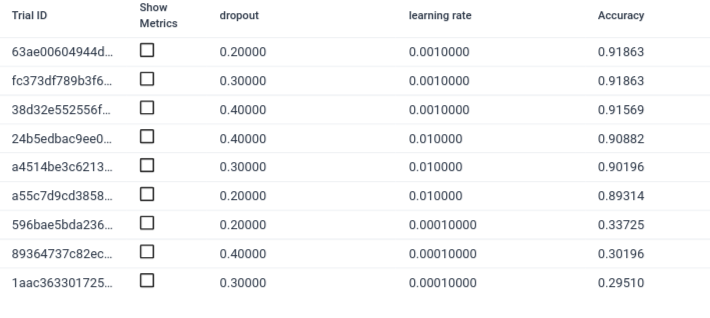
\includegraphics[width=\textwidth]{full_hp.png}
    \caption{Table of full HP training results as seen in TensorBoard.}
    \label{fig:hp_full}
\end{figure}

\subsection{Loss}

\label{subsec:loss}

\begin{figure}[h]\
    \centering
    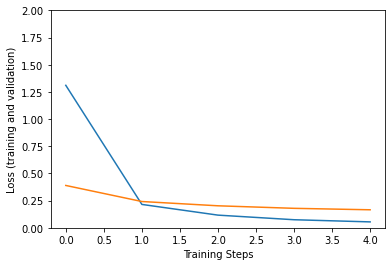
\includegraphics[width=0.6\textwidth]{inception_loss.png}
    \caption{Graph of loss against the number of training steps.}
    \label{fig:incep_loss}
\end{figure}

\section{Requirements}

Sources:
\begin{itemize}
    \item SS: Saahil Shihaz
    \item AD: Android Developers
    \item TF: TensorFlow
    \item MY: Material You
\end{itemize}

Priorities:
\begin{itemize}
    \item H: High
    \item M: Medium
    \item L: Low
\end{itemize}

\subsection{Functional Requirements}
\label{subsec:funcreq}

\begin{table}[h!]
    \begin{tabular}{ |m{1cm}|m{5cm}|m{1.5cm}|m{1.5cm}| }
        \hline
        No. & Description & Source & Priority \\
        \hline
        1 & 
        The app must run on an Android device.
        & SS & H \\
        \hline
        2 & 
        The app must be able to capture an image.
        & SS, AD & H \\
        \hline
        2.1 & 
        The app must be able to display a captured image. 
        & SS, AD & H \\
        \hline
        3 &
        The app must use the Inception V3 model trained in section one to process captured images. 
        & SS, TF & H \\
        \hline
        4 &
        The app must display the guesses produced by the model within 500 milliseconds.
        & SS & H \\
        \hline
        4.1 &
        The app must show the top three guesses as well as their individual percentage probabilities ranked from highest
        to lowest.
        & SS & H \\
        \hline
        4.2 &
        The app should show a small preview of the flowers next to the guesses.
        & SS & M \\
        \hline
        5 & 
        The app must display the time it takes to process an image in milliseconds.
        & SS & H \\
        \hline
        6 &
        The app could contain additional pages that provide more pictures and information about the flower that can be 
        accessed by clicking on the flower's icon.
        & SS & L \\
        \hline
    \end{tabular}
    \label{table:func}
\end{table}
\break
\subsection{Non-functional Requirements}
\label{subsec:nonreq}

\begin{table}[h!]
    \begin{tabular}{ |m{1cm}|m{5cm}|m{1.5cm}|m{1.5cm}| }
        \hline
        No. & Description & Source & Priority \\
        \hline
        1 & 
        The app must function with minimal bugs. 
        & SS & H \\
        \hline
        2 & 
        The app must follow the Material You design specifications.
        & MY & L \\
        \hline
    \end{tabular}
    \label{table:nonfunc}
\end{table}

\subsection{SDK percentage}

\label{subsec:sdk}

\begin{figure}[h]\
    \centering
    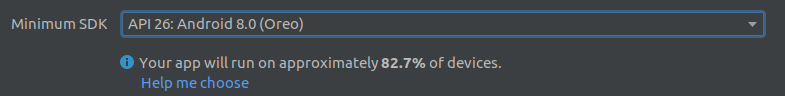
\includegraphics[width=\textwidth]{Min_SDK.png}
    \caption{The percentage of devices that API level 8 will run according to Android Studio.}
    \label{fig:sdk}
\end{figure}

\clearpage

\subsection{Model performance list}

\label{subsec:models}

\begin{figure}[h]\
    \centering
    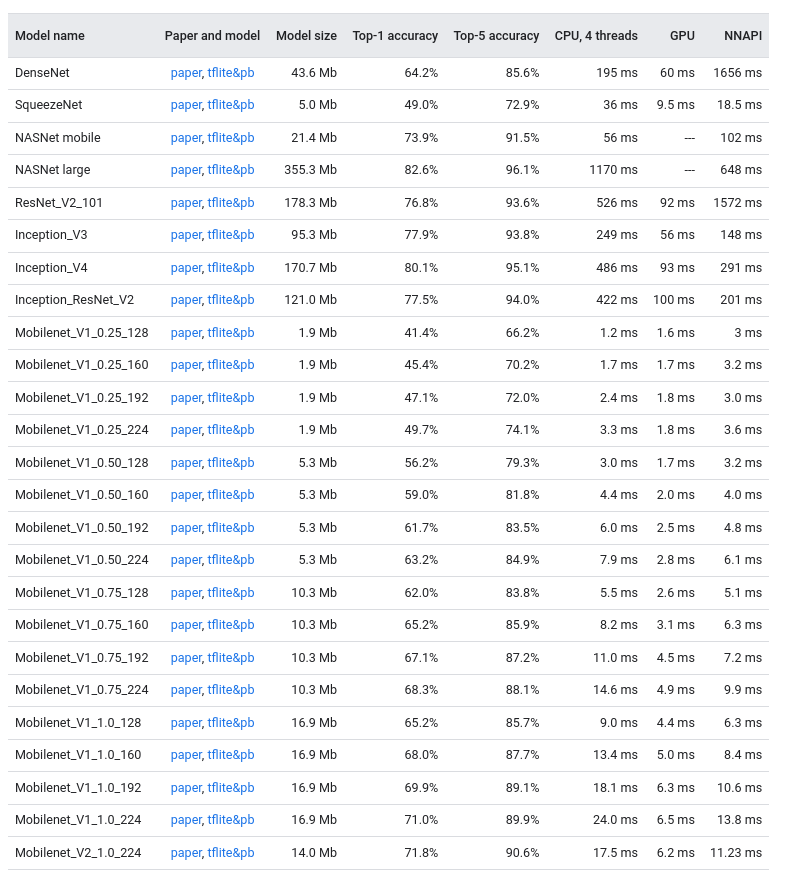
\includegraphics[width=\textwidth]{models.png}
    \caption{The list of models and their performance metrics on the TensorFlow site \cite{TFhostedmodels}.}
    \label{fig:models}
\end{figure}
\clearpage

\section{Testing}
\subsection{Testing device specifications}

\label{subsec:phone_spec}

Samsung Galaxy S20 5G

\par

Apr 27, 2022 5:57

\par

Hardware \\
exynos990 \\
Cores: 8 \\
CPU: \\
2 x M5 \\
2 x Cortex-A76 \\
4 x Cortex-A55 \\
Process: 7 nm LPP \\
Frequencies: \\
442 MHz - 2002 MHz \\
507 MHz - 2504 MHz \\ 
546 MHz - 2730 MHz

\par

GRAPHICS \\
Vendor: ARM \\
GPU: Mali-G77 \\
OpenGL: OpenGL ES 3.2 \\
Max frequency: 800 MHz \\
Resolution: 2400 x 1080 \\
Screen density: 424.48477 ppi \\
Screen size (estimated): 6.2 in / 158 mm

\par

RAM \\
RAM size: 12 GB \\
Type: LPDDR5 2750 MHz \\
Bandwidth: 44 GB/s \\
Channels: 16-bit quad channel

\par

Storage \\
Size: 128 GB \\
Filesystem: sdcardfs \\

\par

DEVICE \\
Model: SM-G981B \\
Codename: x1s \\
Manufacturer: samsung \\
Manufacturing date: October 5, 2020

\par

System \\
Android Version: Android 12 \\
Build: SP1A.210812.016.G981BXXSDFVC9 \\
ROM base: G981BXXSDFVC9 \\
Security patch: April 1, 2022 \\
Architecture: aarch64 (64-bit) \\
Instruction sets: arm64-v8a armeabi-v7a armeabi \\
Kernel: Linux version 4.19.87-23725627 (dpi@21DJ7D03) (Android (dev based on r349610)
clang version 8.0.8 (based on LLVM 8.0.8svn))

\par

Battery \\
Technology: Li-ion \\
Health: Good \\
Capacity (reported by system): 3880 mAh

\par

CAMERA \\
Resolution: 12.2 MP (4032x3024) \\
Focal length: 2.2 mm \\
35mm equivalent focal length: 13.5 mm \\
Sensor size: 5.64 x 4.23 mm \\ 
Crop factor: 6.1x \\
Field of view: 104.1 degrees \\
Pixel size: 1.40 micro metres \\
Aperture: 2.2 \\
Shutter speed: 1/11764 - 1/10 s \\
RAW mode: No \\
ISO sensitivity range: 50 - 3200 \\
RAW mode: Supported \\
Optical image stabilization: No \\
Front camera: 7.1 MP (3216x2208)

\subsection{Results of functionality testing}
\label{subsec:functionality}

\begin{table}[h!]
    \begin{tabular}{ |m{1cm}|m{2cm}|m{2cm}|m{2cm}|m{2cm}| }
        \hline
        Figure & Prediction & Prob. (\%) & Actual & Time (ms) \\
        \hline
        x & Anthurium & 78 & Anthurium & 351 \\
        \hline
        x & Columbine & 48 & Unknown & 376 \\
        \hline
        x & Cyclamen & 47 & Orchid & 364 \\
        \hline
        x & Daffodil & 93 & Daffodil & 378 \\
        \hline
        x & Oxeye Daisy & 96 & Oxeye Daisy & 379 \\
        \hline
        x & Dandelion & 100 & Dandelion & 393 \\
        \hline
        x & Dandelion & 88 & Dandelion & 373 \\
        \hline
        x & Rose & 97 & Rose & 316 \\
        \hline
    \end{tabular}
    \caption{Table of predictions for 8 different flowers found in the vicinity.}
    \label{table:nonfunc}
\end{table}

\subsection{Results of distance testing}
\label{subsec:distance}

\begin{table}[h!]
    \begin{tabular}{ |m{1cm}|m{2.5cm}|m{2cm}|m{2cm}| }
        \hline
        Figure & Distance (cm) & Prediction & Prob. (\%)\\
        \hline
        x & 4 & Rose & 39 \\
        \hline
        x & 15 & Rose & 78 \\
        \hline
        x & 35 & Sword Lily & 56 \\
        \hline
        x & 60 & Carnation & 72 \\ 
        \hline
    \end{tabular}
    \caption{Results from attempting to identify a rose at different distances.}
    \label{table:distance}
\end{table}
\break

\subsection{Results of lighting testing}
\label{subsec:lighting}

\begin{table}[h!]
    \begin{tabular}{ |m{1cm}|m{2.5cm}|m{2cm}|m{2cm}| }
        \hline
        Figure & Lighting (lux) & Prediction & Prob. (\%)\\
        \hline
        x & 2.9 & Rose & 34 \\
        \hline
        x & 25.4 & Rose & 68 \\
        \hline
        x & 5333.6 & Thorn Apple & 45 \\
        \hline
    \end{tabular}
    \caption{Results from attempting to identify a rose at different lighting conditions.}
    \label{table:lighting}
\end{table}
\break

\end{document}